%---------------------------------------------------------------------
\chapter{Einleitung}\label{Ch:Einleitung}
%---------------------------------------------------------------------

%---------------------------------------------------------------------
\section{Motivation}
%---------------------------------------------------------------------

Das Abk�rzungsverzeichnis in der Nomenklatur wird nur erg�nzt, wenn eine Abk�rzung auch tats�chlich verwendet wird, \zB \ac{FFT}, \ac{EC-Motor} oder \ac{HSU}.

Wer jedoch nur das Akronym verwenden m�chte, das dann ebenfalls im Abk�rzungsverzeichnis auftaucht, der kann \verb|\acs| verwenden, \zB \acs{RMS}.

%---------------------------------------------------------------------
\section{Zielsetzung}
%---------------------------------------------------------------------

tbd

\subsection{Tabelle}

\begin{table}[htbp]
    \centering
    \begin{tabular}{|l|l|}
    \hline
    Test & Tester \\ \hline
    1 & 2 \\ \hline
    4 & 3 \\ \hline
    \end{tabular}
    \caption{Tabelle als Beispiel}
\end{table}

\subsection{Image}


\begin{figure}[htbp]
    \centering
    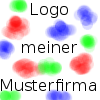
\includegraphics[width=.8\textwidth]{bilder/example/example.png}
    \caption{Ein Bild Beispiel}
\end{figure}
